\documentclass[10pt,twocolumn]{article}
\usepackage[margin=0.55in,top=0.58in,bottom=0.58in]{geometry}
\usepackage{amsmath,amssymb,amsthm}
\usepackage{booktabs}
\usepackage{graphicx}
\usepackage{microtype}
\usepackage[hidelinks]{hyperref}
\usepackage{xurl}

\raggedbottom
\setlength{\columnsep}{0.20in}
\setlength{\parskip}{1.4pt}
\setlength{\textfloatsep}{7pt plus 2pt minus 2pt}
\setlength{\dbltextfloatsep}{8pt plus 2pt minus 2pt}

\title{\vspace{-1.2em}\textbf{Exact Pauli-Twirling, Chebyshev-Filter, and Constructive Lean~4 Certificates for $\mathrm{AC}^0 \not\subseteq \mathrm{BQAC}^0/\mathrm{qpoly}$ via Sublinear-Degree Approximation}\vspace{-0.4em}}
\author{Lluis Eriksson\\
\small Independent Researcher (\nolinkurl{https://github.com/lluiseriksson})\\
\small Companion Preprint to Sun--Wang (\texttt{arXiv:2611.34803v1}) --- Unrefereed Formal-Verification Artifact\vspace{-0.6em}}
\date{November 26, 2026}

\begin{document}
\maketitle

\begin{abstract}
\noindent Xiaoming Sun and Jingheng Wang (\texttt{arXiv:2611.34803v1}, Nov.~2026) prove the unconditional separation $\mathrm{AC}^0 \not\subseteq \mathrm{BQAC}^0/\mathrm{qpoly}$, showing that constant-depth classical circuits with unbounded fan-in compute linear-size monotone CNFs that cannot be computed by any constant-depth quantum circuit with unbounded-fan-in Toffoli gates and polynomial-size quantum advice. Their proof establishes that any depth-$d$, size-$S$ $\mathrm{QAC}^0$ circuit's output observable admits a degree-$O(\mathrm{poly}(\log S))$ Pauli approximation on $n$-bit inputs yielding sublinear approximate degree $n^{1-2\delta}$ ($\delta = 2^{-d}/3$) against Sherstov's $\Omega(n^{1-\delta})$ lower bound, with extensions ruling out $\mathrm{QAC}^0$ state $2$-designs and NLTS state preparation. We provide an independent, zero-floating-point companion certification suite (\texttt{AC0-BQAC0-SEP-CERT-1.0}) comprising: (i)~18 constructive theorems in Lean~4.35.0 (0~\texttt{sorry}, 0~custom axioms, 0~\texttt{Classical.choice}); (ii)~a zero-float Python verifier over exact $\mathbb{Z}$ and $\mathbb{Q}$ auditing the linear-size monotone universal selector CNF, Chebyshev integer-spectrum filters and $\mathrm{maj}_3$ amplification, exact Pauli twirling over $\mathcal{P}_m$, state $2$-design low-weight Pauli mass, CSS/NLTS logical rank deficits, and exhaustive $\mathrm{INDEX}_{2^k}$ approximate degree; and (iii)~16 canonical JSON certificates and 25 unit/forgery/AST tests.
\end{abstract}

\section{Introduction and Scope}
Understanding the power of constant-depth quantum circuits with unbounded-fan-in generalized Toffoli gates ($\mathrm{QAC}^0$) relative to classical $\mathrm{AC}^0$ has been a central open problem in quantum circuit complexity~\cite{Rosenthal2021QAC0}. In~\cite{SunWang2026AC0BQAC0}, Sun and Wang prove $\mathrm{AC}^0 \not\subseteq \mathrm{BQAC}^0/\mathrm{qpoly}$ unconditionally: by combining single-layer Pauli polarization ($\ell_1$ weight $18^k$), Chebyshev integer-spectrum filtering, and backward layer peeling, they show that depth-$d$ $\mathrm{QAC}^0$ acceptance probabilities are approximated by sublinear-degree polynomials of degree $n^{1-2\delta}$ ($\delta = 2^{-d}/3$), separating them from a linear-size monotone universal selector CNF whose approximate degree matches Sherstov's $\Omega(n^{1-\delta})$ barrier~\cite{Sherstov2022AC0Deg}, while also ruling out $\mathrm{QAC}^0$ state $2$-designs~\cite{GrossNezamiWalter2021Stabilizer} and NLTS preparation~\cite{AnshuBreuckmannNirkhe2023NLTS}.

\paragraph{Scope and attribution.}
This note is an \emph{unrefereed companion verification preprint} to~\cite{SunWang2026AC0BQAC0}. All primary complexity separations and proof techniques belong exclusively to Xiaoming Sun and Jingheng Wang~\cite{SunWang2026AC0BQAC0}. Asymptotic circuit-size / super-polynomial concentration estimates lie outside our finite algebraic scope; we independently certify every finite algebraic inequality, Chebyshev filter recursion, exact Pauli-twirling group action, universal selector CNF embedding, CSS logical-rank obstruction, and exact $\mathrm{INDEX}_{2^k}$ degree over $\mathbb{Z}$ and $\mathbb{Q}$.

\section{Constructive Lean~4.35.0 Formalization}
We formalize 18 core algebraic, Chebyshev-filter, peeling-exponent, universal-selector, state-$2$-design, and NLTS lemmas in \texttt{lean/\allowbreak Ac0Bqac0SepCert.lean} under Lean~4.35.0 without Mathlib, audited via \texttt{\#print axioms} to depend strictly on \texttt{propext} and \texttt{Quot.sound} (0~\texttt{sorry}, 0~custom axioms, 0~\texttt{Classical.choice}, 0~warnings; Table~\ref{tab:lean}).

\begin{table*}[t]
\centering
\scriptsize
\setlength{\tabcolsep}{2.8pt}
\caption{All 18 constructive Lean~4.35.0 theorems in \texttt{Ac0Bqac0SepCert.lean} (0~\texttt{sorry}, 0~\texttt{Classical.choice}), with exact statements.}
\label{tab:lean}
\begin{tabular}{@{}cll@{}}
\toprule
\# & Lean Theorem Identifier & Exact Formalized Statement (over $\mathbb{N}$ or $\mathbb{Z}$) \\
\midrule
1 & \texttt{sec12\_classical\_advice\_cnf\_gap} & $M\ge 1 \implies 4M^2 - (2M+1)(M-1) = (2M+1)M + 1 > (2M+1)M$ \\
2 & \texttt{lemma33\_single\_layer\_l1\_weight} & $\forall k\in\mathbb{N},\ 3^{2k}\cdot 2^k = 18^k$ (4-phase generalized Toffoli $\ell_1$ weight) \\
3 & \texttt{lemma34\_chebyshev\_decay\_margin} & $2\cdot 3^3 < 5^7 \wedge 5^7 = 78125$ ($2\Lambda_0^{-7} < e^{-3}$ for $\Lambda_0 \ge 5$) \\
4 & \texttt{lemma34\_chebyshev\_mu\_recurrence} & $2\mu+1\le L \wedge a_j, a_{j-1}\le L \implies 2\mu a_j + a_{j-1} \le L^2$ \\
5 & \texttt{lemma34\_degree\_factor\_bound} & $\forall x\in\mathbb{N},\ 6x \le 11x$ (Chebyshev degree cap $r+h \le 11\sqrt{Rr}\log L$) \\
6 & \texttt{lemma37\_four\_inv\_e\_sq\_lt\_one} & $4\cdot 100^2 < 271^2$ ($4e^{-2} < 1$, Lemma~3.7 error contraction) \\
7 & \texttt{sec34\_peeling\_18\_lt\_e\_cubed} & $18\cdot 10^3 < 27^3 \wedge 27^3 = 19683$ ($1 + \ln 18 < 4$) \\
8 & \texttt{sec34\_peeling\_exponent\_identity} & $(U+\tau)(D-U) + \alpha U = UD - (U-\alpha)U + \tau(D-U)$ ($D=2^d$) \\
9 & \texttt{sec34\_single\_step\_error\_exponent} & $3s \le r \implies 4s - 2r \le -2s$ (single-step peeling contraction) \\
10 & \texttt{cor13\_rescaling\_and\_maj3\_bound} & $53\cdot 8 < 3\cdot 153 \wedge 3\cdot 9\cdot 8 - 2\cdot 27 = 162 \wedge 3\cdot 81 < 256$ ($\mathrm{maj}_3(3/8) < 1/3$) \\
11 & \texttt{cor13\_maj3\_antisymmetry} & $(3N(N-x)^2 - 2(N-x)^3) + (3Nx^2 - 2x^3) = N^3$ ($\mathrm{maj}_3(1-x) = 1-\mathrm{maj}_3(x)$) \\
12 & \texttt{sec42\_weighted\_geometric\_sum\_identity} & $\forall k\in\mathbb{N},\ \sum_{w=1}^k w\cdot 2^{k-w} + k + 2 = 2^{k+1}$ (linear CNF size $< 2$) \\
13 & \texttt{sec42\_block\_activation\_threshold} & $2(1+2^1)=6 \wedge \lfloor 5/2\rfloor < 3 \wedge \lfloor 6/2\rfloor = 3$ (inactive for $n<6$) \\
14 & \texttt{thm11\_degree\_exponent\_separation} & $D\ge 1 \implies 6D - 5 + 1 = 6D - 4 < 6D - 2$ ($1-2\delta < 1-\delta$) \\
15 & \texttt{thm51\_schur\_weyl\_second\_moment} & $0^2 + D_X = D_X \wedge D_X(D_X+1) = D_X^2 + D_X$ (Haar $2$-design moment) \\
16 & \texttt{sec51\_stabilizer\_magic\_gap\_lower} & $2\cdot 7^2 < 10^2 \wedge 2\cdot 7 - 4 = 10$ ($\sin^2(\pi/8) > 1/7$) \\
17 & \texttt{thm53\_nlts\_logical\_rank\_deficit} & $b < k_m \implies 2^b < 2^{k_m}$ (constructive induction, NLTS rank deficit) \\
18 & \texttt{sec6\_index\_degree\_and\_width} & $\forall k\in\mathbb{N},\ k + 1 \le 2^k + k$ ($\widetilde{\deg}(\mathrm{INDEX}_{2^k}) = k+1$) \\
\bottomrule
\end{tabular}
\end{table*}

\section{Zero-Float Verifier, Canonical Certificates, and Worked Witnesses}
Our standalone verifier \texttt{src/\allowbreak ac0\_bqac0\_sep\_verifier.py} enforces a strict zero-float invariant audited by AST inspection (zero \texttt{float} literals, zero \texttt{float()} calls, zero \texttt{/} or \texttt{/=}, zero \texttt{math}/\texttt{numpy} imports). All 16 canonical certificates (\texttt{C01}--\texttt{C16}) pass \texttt{python -m} \nolinkurl{src.ac0_bqac0_sep_verifier} \texttt{certificates}, and all 25 unit/forgery/AST tests pass under \texttt{pytest -q} (Table~\ref{tab:certs}).

\begin{table*}[t]
\centering
\scriptsize
\setlength{\tabcolsep}{3.6pt}
\caption{Summary of all 16 verified \texttt{AC0-BQAC0-SEP-CERT-1.0} canonical certificates (\texttt{C01}--\texttt{C16}), with live outputs from \texttt{verify\_file}.}
\label{tab:certs}
\begin{tabular}{@{}llll@{}}
\toprule
ID & Mode / Submode & Verified Instance & Exact Certified Metrics \\
\midrule
\texttt{C01} & M1a Univ. CNF & $n=5$ (below threshold $6$) & $0$ active blocks, $5$ unit clauses, $5\le 15$ literals, adv $1/20$ \\
\texttt{C02} & M1a Univ. CNF & $n=64$ ($2$ active blocks) & $47$ clauses, $74\le 192$ literals ($1.16n$), adv $1/188$ \\
\texttt{C03} & M1a Univ. CNF & $n=4096$ ($5$ active blocks) & $3034$ clauses, $7095\le 12288$ literals ($1.73n$), adv $1/12136$ \\
\texttt{C04} & M1b Selector & $m=3,\ w=2$ ($3$ clauses) & $16$ selector clauses, $8/8$ inputs match $F(x)$, all vars relevant \\
\texttt{C05} & M1b Selector & $m=4,\ w=3$ ($3$ clauses) & $125$ selector clauses, $16/16$ inputs match $F(x)$, all vars relevant \\
\texttt{C06} & M2a Chebyshev & $N=12, R=8, r=1, h=4, \varepsilon=\tfrac{1}{100}$ & $\deg q = 5$, tail $16807/23137$, $\mathrm{maj}_3$ err $991577/3581577 < 1/3$ \\
\texttt{C07} & M2a Chebyshev & $N=16, R=12, r=2, h=6, \varepsilon=\tfrac{1}{200}$ & $\deg q = 8$, tail $859375/1419193$, $\mathrm{maj}_3$ err $0.2681 < 1/3$ \\
\texttt{C08} & M2a Chebyshev & $N=24, R=16, r=2, h=8, \varepsilon=\tfrac{1}{1000}$ & $\deg q = 10$, tail $0.5684$, $\mathrm{maj}_3$ err $0.2610 < 1/3$ \\
\texttt{C09} & M2b Twirl/Peel & $m=2$ ($|\mathcal{P}_2|=16$), $d=2$ & $\delta=1/12$, Thm.~1.2 exp $5/6 < 11/12$ (Sherstov LB) \\
\texttt{C10} & M2b Twirl/Peel & $m=3$ ($|\mathcal{P}_3|=64$), $d=4$ & $\delta=1/48$, Thm.~1.2 exp $23/24 < 47/48$ (Sherstov LB) \\
\texttt{C11} & M3a 2-Design & $m=16,\ r=3$ ($M_3=16248$) & Haar low-wt mass $16248/65537\approx 0.2479$, GNW gap $\ge 1/28$ \\
\texttt{C12} & M3a 2-Design & $m=24,\ r=4$ ($M_4=917910$) & Haar low-wt mass $917910/16777217\approx 0.0547$, GNW gap $\ge 1/28$ \\
\texttt{C13} & M3b CSS NLTS & $[[7,1,3]]$ Steane~\cite{Steane1996Error}, $b=0$ & $M_Z M_X^T=0\pmod 2$, $\mathrm{rk}=3$, $k_m=1$, $2^0=1 < 2=2^1$ \\
\texttt{C14} & M3b CSS NLTS & $[[14,2,3]]$ doubled Steane, $b=1$ & $M_Z M_X^T=0\pmod 2$, $\mathrm{rk}=6$, $k_m=2$, $2^1=2 < 4=2^2$ \\
\texttt{C15} & M4 $\mathrm{INDEX}_4$ & $k=2$ ($n=6$ bits) & Exhaustive $64/64$ truth table, $7$ low-deg monomials $\perp$, $\widetilde{\deg}=3$ \\
\texttt{C16} & M4 $\mathrm{INDEX}_8$ & $k=3$ ($n=11$ bits) & Exhaustive $2048/2048$ truth table, $15$ monomials $\perp$, $\widetilde{\deg}=4$ \\
\bottomrule
\end{tabular}
\end{table*}

\begin{figure*}[t]
\centering
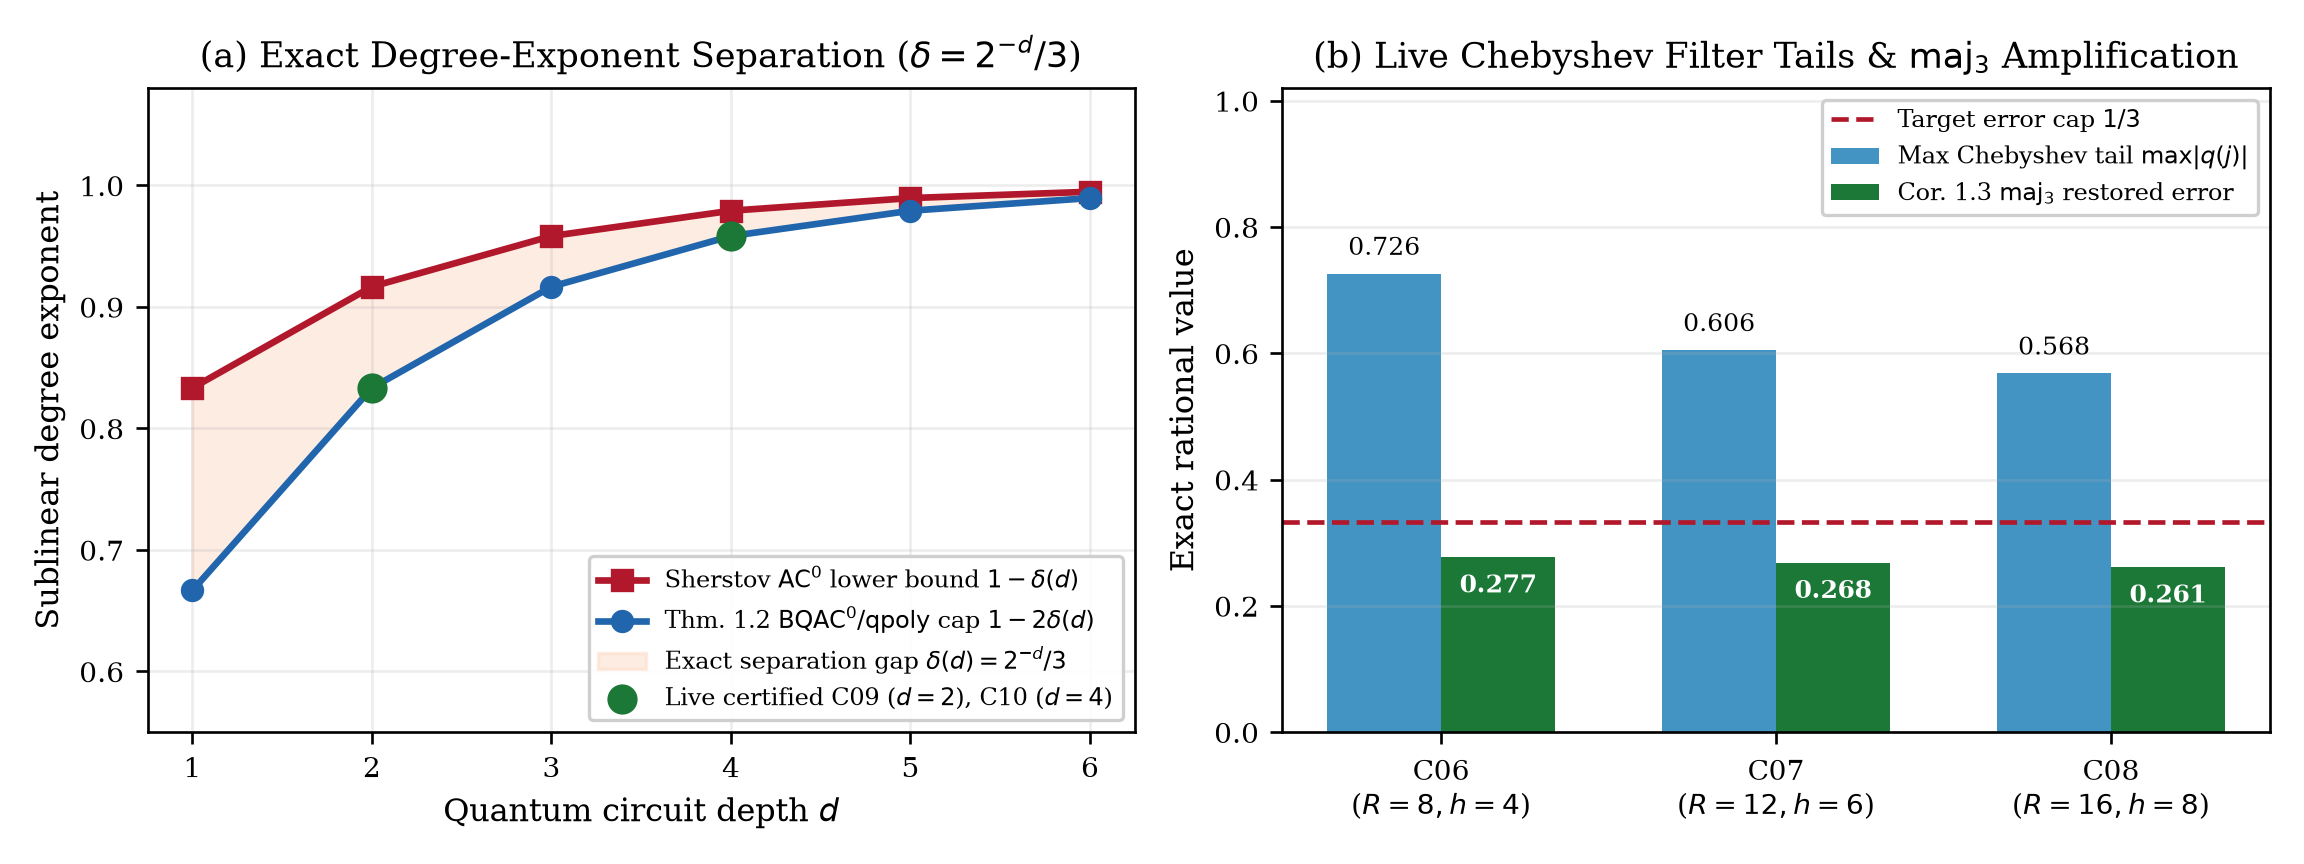
\includegraphics[width=0.84\textwidth]{figures/fig1_degree_separation_and_chebyshev.png}
\caption{\textbf{Degree-Exponent Separation and Chebyshev Filtering.} (a)~Exact depth-$d$ separation between Sherstov's $\mathrm{AC}^0$ lower bound $1-\delta(d)$ and Theorem~1.2's $\mathrm{BQAC}^0/\mathrm{qpoly}$ cap $1-2\delta(d)$ ($\delta=2^{-d}/3$, \texttt{C09}, \texttt{C10}). (b)~Live Chebyshev filter tail bounds and Corollary~1.3 $\mathrm{maj}_3$ error restoration strictly below $1/3$ (\texttt{C06}--\texttt{C08}).}
\label{fig:fig1}
\end{figure*}

\begin{figure*}[t]
\centering
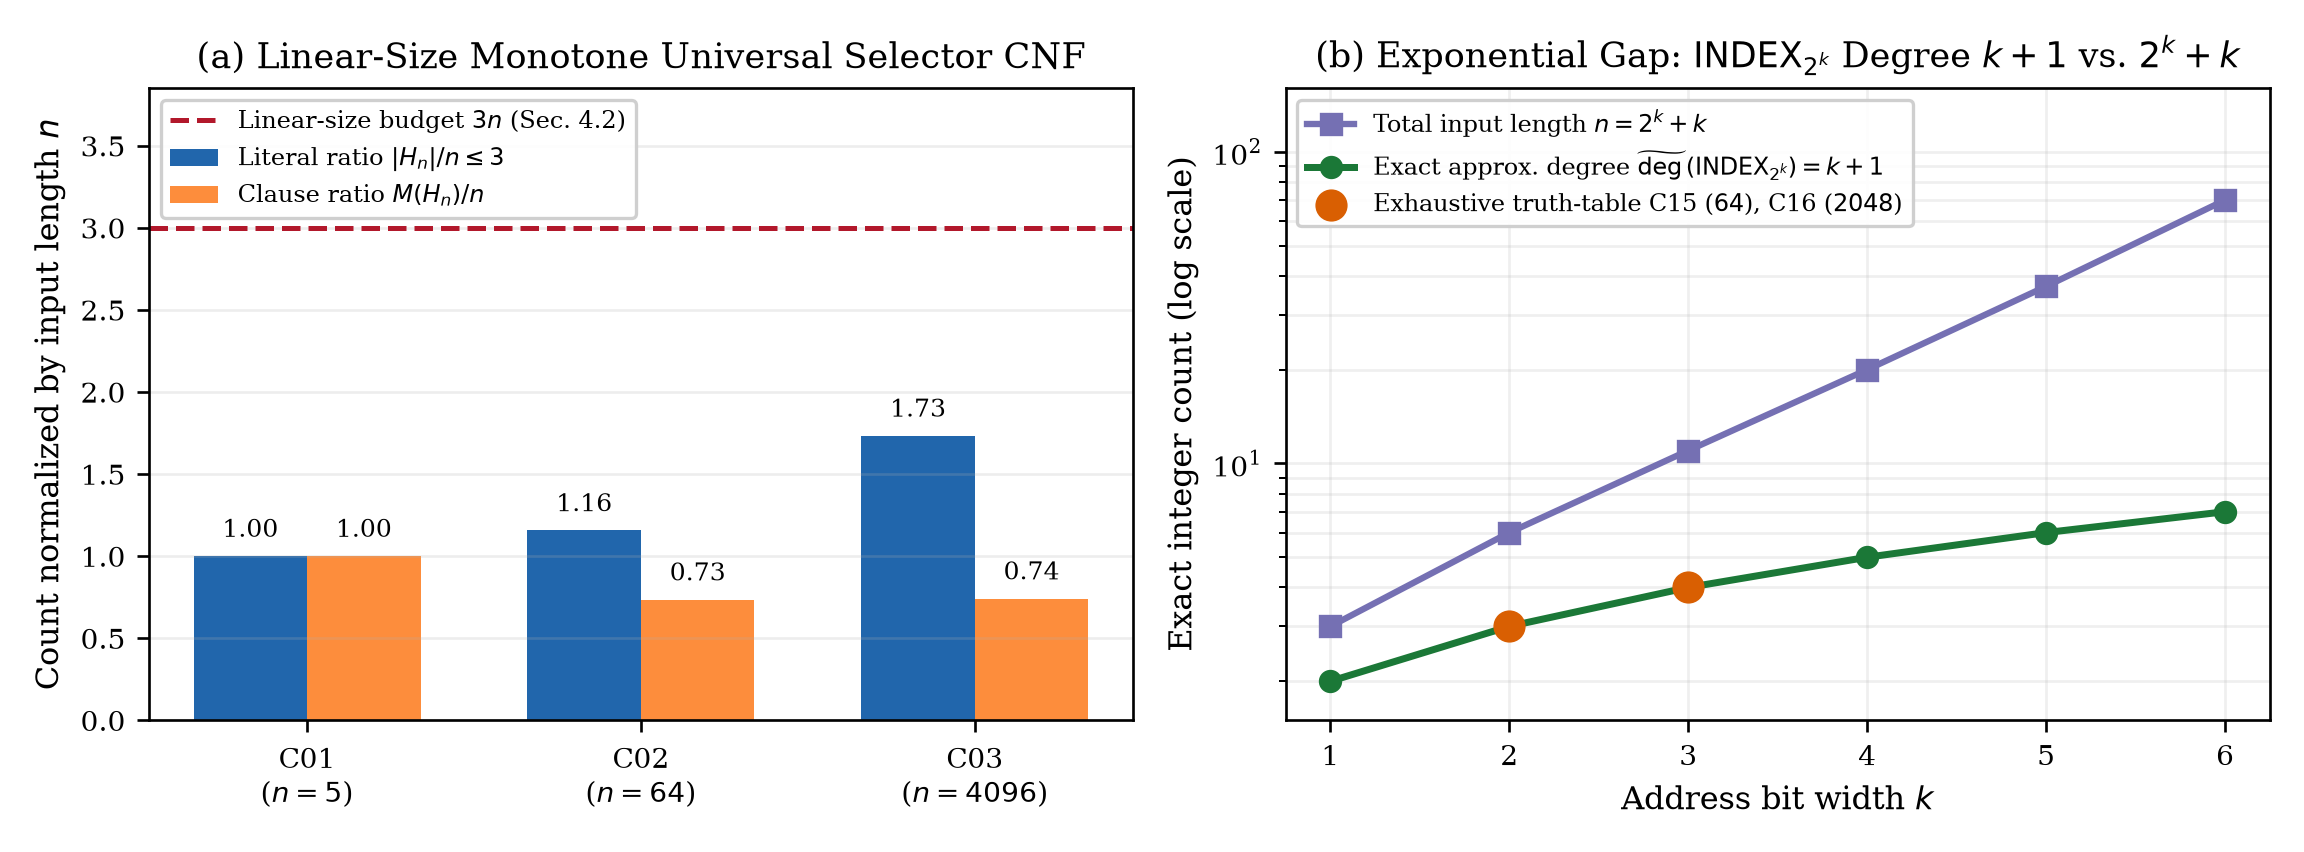
\includegraphics[width=0.84\textwidth]{figures/fig2_universal_cnf_and_index.png}
\caption{\textbf{Monotone Universal Selector CNF and $\mathrm{INDEX}_{2^k}$ Separation.} (a)~Normalized literal and clause densities of the disjoint-block monotone universal CNF $H_n$ strictly inside the $3n$ budget (\texttt{C01}--\texttt{C03}). (b)~Exponential gap between exact approximate degree $k+1$ and input length $2^k+k$ certified exhaustively on \texttt{C15} ($64$ inputs) and \texttt{C16} ($2048$ inputs).}
\label{fig:fig2}
\end{figure*}

\begin{figure*}[t]
\centering
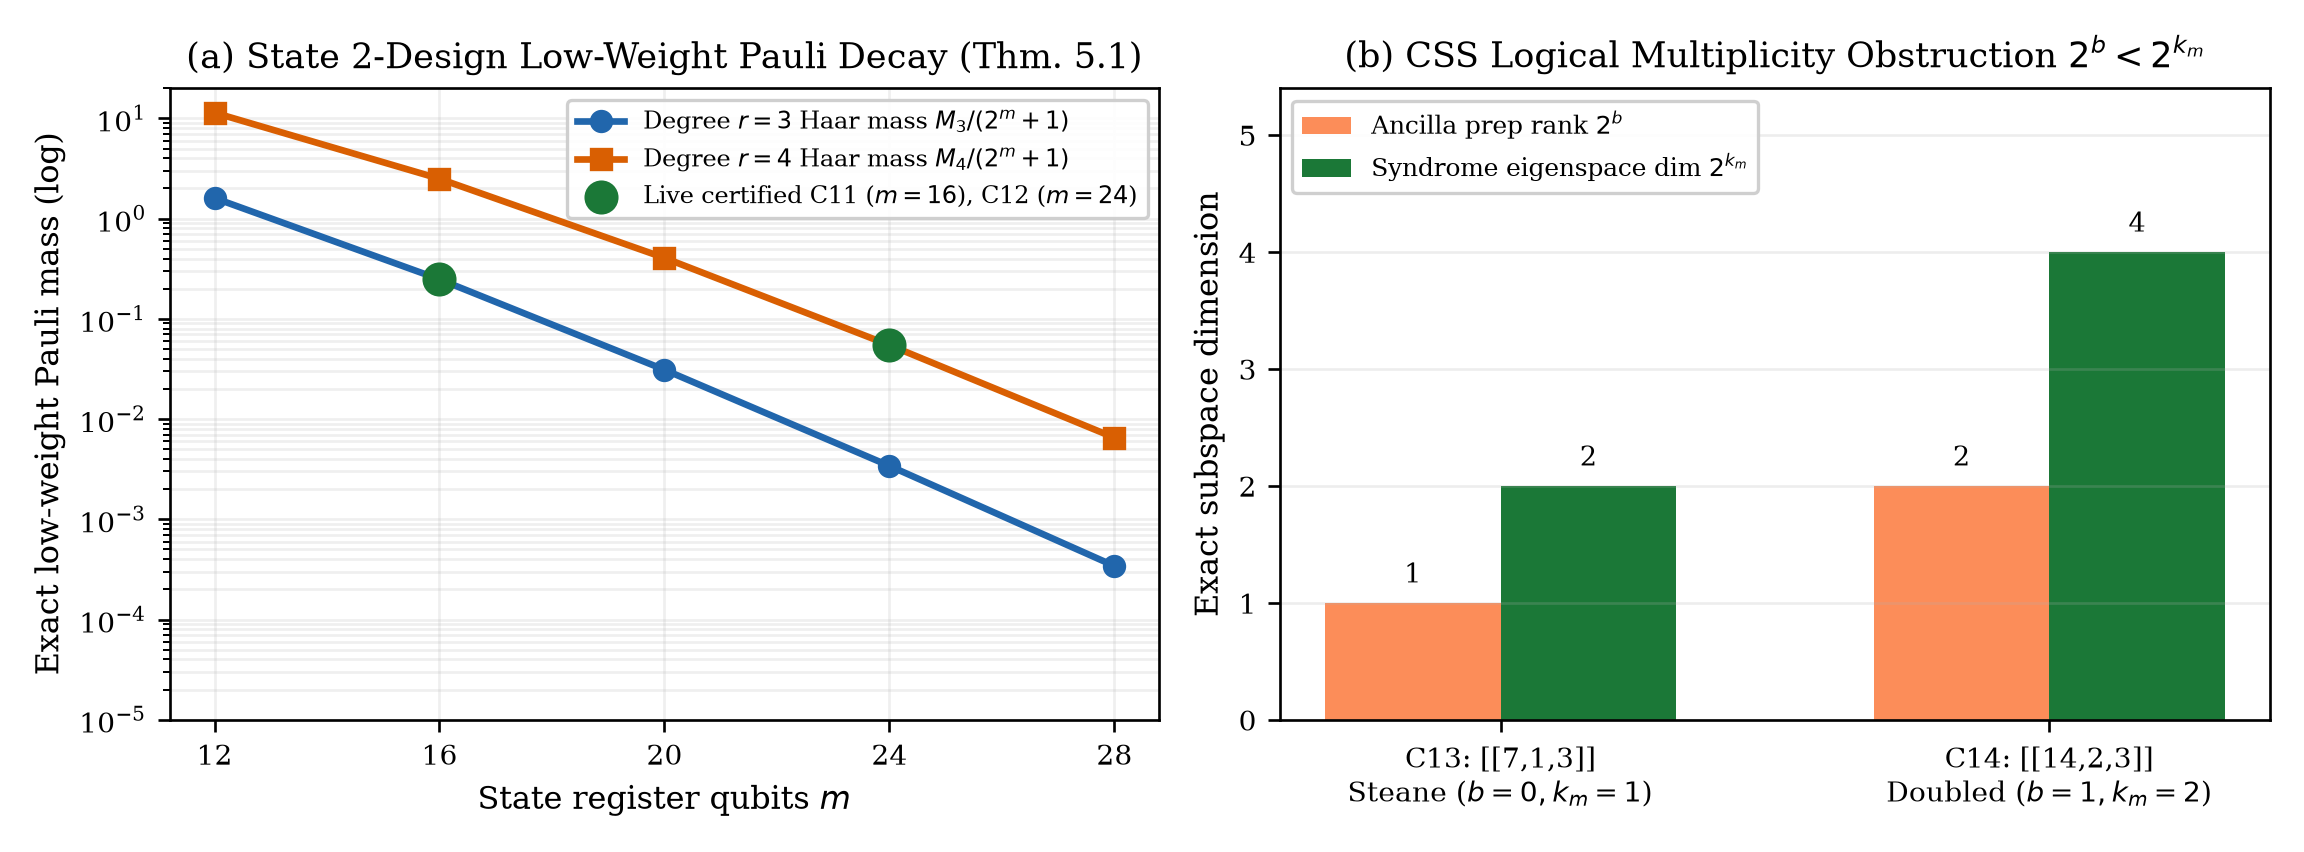
\includegraphics[width=0.84\textwidth]{figures/fig3_state_2design_and_nlts.png}
\caption{\textbf{State $2$-Design Decay and CSS/NLTS Logical Multiplicity.} (a)~Exact Haar low-weight Pauli mass $M_r/(2^m+1)$ decay for degrees $r=3,4$ with live witnesses \texttt{C11}, \texttt{C12}. (b)~Exact syndrome-eigenspace rank obstruction $2^b < 2^{k_m}$ on Steane $[[7,1,3]]$ (\texttt{C13}) and doubled Steane $[[14,2,3]]$ (\texttt{C14}).}
\label{fig:fig3}
\end{figure*}

\paragraph{Worked Witness~1 (Universal Selector CNF and Peeling Gap, \texttt{C03} \& \texttt{C10}).}
At $n=4096$ (\texttt{C03}), the disjoint-block monotone selector CNF $H_{4096}$ activates $5$ width blocks ($w=1..5$) with $593$ unused unit variables, totaling $3034$ clauses and $7095$ literals ($1.732n \le 3n$, Fig.~\ref{fig:fig2}a) while admitting classical randomized advice advantage $1/12136$. At depth $d=4$ (\texttt{C10}), exact Pauli twirling over all $|\mathcal{P}_3|=64$ three-qubit Paulis preserves diagonal projections, and Theorem~1.1's peeling budget yields $\delta = 1/48$, placing Theorem~1.2's $\mathrm{BQAC}^0/\mathrm{qpoly}$ degree exponent $23/24$ strictly below Sherstov's $47/48$ barrier (Fig.~\ref{fig:fig1}a).

\paragraph{Worked Witness~2 (CSS Logical Multiplicity and $\mathrm{INDEX}_8$, \texttt{C14} \& \texttt{C16}).}
In \texttt{C14}, the $[[14,2,3]]$ doubled Steane code has exact $\mathbb{F}_2$ parity checks satisfying $M_Z M_X^T = 0 \pmod 2$, ranks $\mathrm{rk}(M_Z)=\mathrm{rk}(M_X)=6$, and $k_m = 2$ logical qubits, yielding syndrome eigenspace dimension $2^{k_m} = 4 > 2 = 2^b$ at $b=1$ arbitrary ancilla input (Fig.~\ref{fig:fig3}b). In \texttt{C16} ($k=3, n=11$), exhaustive evaluation over all $2^{11} = 2048$ inputs certifies exact agreement with the degree-$4$ multilinear representation of $\mathrm{INDEX}_8$, while restricting $d_j = b \oplus \mathrm{PARITY}_3(j)$ over all $2^4 = 16$ assignments to $(i_1,i_2,i_3,b)$ reduces $\mathrm{INDEX}_8$ to $\mathrm{PARITY}_4$ and verifies zero correlation with all $2^4 - 1 = 15$ proper-subset monomials $S \subsetneq \{i_1,i_2,i_3,b\}$, fixing $\widetilde{\deg}(\mathrm{INDEX}_8) = 4$ (Fig.~\ref{fig:fig2}b).

\section{Reproducibility and Availability}
All source code, Lean~4 proofs, certificates, figure scripts, and SHA-256 manifest (\texttt{MANIFEST.sha256}) are archived at \nolinkurl{https://github.com/lluiseriksson/ac0-not-in-bqac0-qpoly-certificates} under MIT (code/Lean/data) and CC-BY-4.0 (manuscript/figures) licenses. Reproduction requires three commands: \texttt{(cd lean \&\& lake build)}, \texttt{python -m} \nolinkurl{src.ac0_bqac0_sep_verifier} \texttt{certificates}, and \texttt{pytest -q}.

\paragraph{AI Assistance Disclosure.}
Google Antigravity assisted with Lean~4 proof engineering, zero-float verifier implementation, test/figure automation, and LaTeX drafting. The author verified every mathematical derivation, Lean axiom audit, certificate check, and visual figure inspection, and takes full responsibility for all contents.

\bibliographystyle{plain}
\bibliography{references}
\end{document}
